\chapter{Soft Actor-Critic}

% https://blog.csdn.net/weixin_44436360/article/details/108077422
% https://zhuanlan.zhihu.com/p/70360272

Robot Learning正在快速的发展,其中深度强化学习deep reinforcement learning(DRL),
特别是面向连续控制continous control的DRL算法起着重要的作用。
在这一领域中,目前有三类行之有效的modle free DRL算法:
\begin{itemize}
%\setlength{\itemsep}{0pt}
%\setlength{\parsep}{0pt}
\setlength{\parskip}{0pt}
\item[-]
TRPO,PPO
\item[-]
DDPG及其拓展(D4PG,TD3等)
\item[-]
Soft Q-Learning, Soft Actor-Critic
\end{itemize}


PPO算法是主流的DRL算法,同时面向离散控制和连续控制,在OpenAI Five上取得了巨大成功。
但是PPO是一种on-policy算法,存在sample inefficiency的缺点,需要巨量的采样才能学习。
DDPG及其拓展是面向连续控制的off-policy的算法,相对于PPO来说更sample efficient,
但是它存在对其超参数敏感,收敛效果差的问题。DDPG训练的是一种确定性策略deterministic policy,
即每一个state下都只考虑最优的一个动作。DDPG的拓展版D4PG从paper中的结果看取得了非常好的效果,
但是并没有开源,目前github上也没有人能够完全复现Deepmind的效果。

SAC算法是面向最大熵强化学习开发的一种off-policy算法。
与DDPG相比,SAC使用的是随机策略,相比确定性策略具有一定的优势。
Soft Actor-Critic在公开的benchmark中取得了非常好的效果,并且能直接应用到真实机器人上。
最关键的是,Soft Actor-Critic是完全开源的,因此,深入理解Soft Actor-Critic 算法具有非常重要的意义。

\subsection{相关链接}

Papers:
\begin{itemize}
%\setlength{\itemsep}{0pt}
%\setlength{\parsep}{0pt}
\setlength{\parskip}{0pt}
\item[-]
\href{https://arxiv.org/abs/1801.01290}{Soft Actor-Critic: 
Off-Policy Maximum Entropy Deep Reinforcement Learning with a Stochastic Actor}
\item[-]
\href{https://arxiv.org/abs/1812.05905}{Soft Actor-Critic Algorithms and Applications}
\item[-]
\href{https://arxiv.org/abs/1702.08165}{Reinforcement Learning with Deep Energy-Based Policies (Soft Q-Learning)}
\end{itemize}

Codes:
\begin{itemize}
%\setlength{\itemsep}{0pt}
%\setlength{\parsep}{0pt}
\setlength{\parskip}{0pt}
\item[-]
\href{https://github.com/rail-berkeley/softlearning}{rail-berkeley/softlearning (原作者实现)}
\item[-]
\href{https://github.com/vitchyr/rlkit}{vitchyr/rlkit}
\item[-]
\href{https://github.com/openai/spinningup}{openai/spinningup}
\item[-]
\href{https://github.com/hill-a/stable-baselines}{hill-a/stable-baselines}
\end{itemize}


\section{SAC}

% \noindent 最大熵强化学习算法SAC \\
% https://www.toutiao.com/article/6845540775015481870/

SAC:Soft Actor-Critic,Off-Policy Maximum Entropy Deep Reinforcement 
Learning with a Stochastic Actor。


\subsection{模型结构}

模型同时学习action value Q、state value V和policy $\pi$。

V中引入Target V,供Q学习时使用;Target Network使学习有章可循、效率更高。

Q有两个单独的网络,选取最小值供V和$\pi$学习时使用,希望{\bf 减弱$Q$的过高估计}。

$\pi$学习的是分布的参数:均值和标准差;这与DDPG不同,DDPG的$\pi$是Deterministic的,
输出直接就是action,而{\bf SAC学习的是个分布},学习时action需要从分布中采样,
是{\bf Stochastic}的。

\begin{figure}[!htb]
\centering
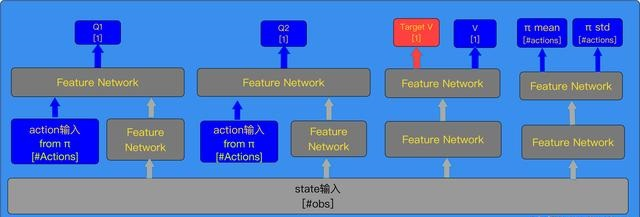
\includegraphics[scale=1.0]{pix/sac.jpg}
\caption{SAC}
%\label{fig:label}
\end{figure}


\subsection{Soft}

Soft,Smoothing,Stable。

原始的强化学习的目标是最大化累计reward:
\begin{equation}\label{rl_objective_function}
\sum_t\mathbb{E}_{(s_t,a_t)\sim\rho_\pi}\left[r(s_t, a_t)\right]
\end{equation}
其学习目标很直接,就是学习一个policy使得累加的reward期望值最大:
\begin{equation}\label{rl_reward_function}
\pi^* = \arg\max_\pi \mathbb{E}_{(s_t,a_t)\sim\rho_\pi}
\Big[ \sum_t r(s_t, a_t) \Big]
\end{equation}

\noindent 而强化学习最大熵目标函数(maximum entropy objective)则如下,比上面这个最初的累计奖赏,
增加了policy $\pi$的每一次输出的action的信息熵:

\begin{equation}\label{maximum_entropy_objective}
\pi^* = \arg\max_\pi \mathbb{E}_{(s_t,a_t)\sim\rho_\pi}
\Big[ \sum_t \big(
\underbrace{r(s_t, a_t)}_{\text{reward}} + 
\underbrace{\alpha \mathcal{H}(\pi(\cdot | s_t))}_{\text{entropy}}
\big)\Big]
\end{equation}
上式中的$\alpha$确定了熵项对于奖励的相对重要性。
与传统的DRL学习目标不同,不仅想要长期的回报最大,
还想要policy的每一次输出的action的熵最大。这样做其实就是为了让策略随机化,
即输出的每一个action的概率尽可能分散,而不是集中在一个action上。
也是在鼓励探索,为具有相似的$Q$值的动作分配近乎均等的概率,
不会给动作范围内任何一个动作分配非常高的概率,避免了反复选择同一个动作而陷入次优。
同时通过最大化奖赏,放弃明显没有前途的策略(放弃低奖赏策略)。
总的来说,具有以下几个优势:
\begin{itemize}
%\setlength{\itemsep}{0pt}
%\setlength{\parsep}{0pt}
\setlength{\parskip}{0pt}
\item[(1)]
更强的探索能力;
\item[(2)]
更鲁棒,面对干扰的时候能更容易做出调整;
\item[(3)]
训练速度加快(最大熵使探索更加均匀)。
\end{itemize}

A3C目标函数里的熵正则项和形式一样,只是作为正则项,系数很小。

\begin{equation}\label{entropy_of_policy}
J(\pi) = \sum_{t=0}^{T-1} \mathbb{E}_{(s_t,a_t)\sim\rho_\pi}
[r(s_t, a_t) + \alpha \mathcal{H}(\pi(\cdot | s_t))]
\end{equation}


\subsection{soft policy evaluation}

\cite{YZhang2020}
\parencite{YZhang2020}


对于一个固定的策略$\pi$, 在Soft Policy Iteration中,
近似{\bf soft $Q$-value}可以通过Bellman backup算子迭代出来,迭代更新规则如下:
\begin{equation}\label{soft_policy_evaluation}
\mathcal{T}^\pi Q(s_t, a_t) \triangleq r(s_t, a_t) 
+ \gamma \mathbb{E}_{s_{t+1}\sim\rho_s} [V^\pi(s_{t+1})],
\end{equation}
上式即是所谓的Bellman backup operator,作用范围为算子
$Q: \mathcal{S} \times \mathcal{A} \rightarrow \mathcal{R}$,
其中$V^\pi(s)$为soft state value function:
$$
V^\pi(s_t) = \mathbb{E}_{a_t\sim\pi}[Q^\pi(s_t,a_t)-\alpha\log\pi(a_t|s_t)].
$$
\begin{emp_box}
上式中的$\alpha$在大多数文献中并未出现,具体原因待查。
\end{emp_box}
If we define the entropy augmented reward as
$$
r_\pi(s_t,a_t) \triangleq r(s_t, a_t) 
+ \alpha\gamma \mathbb{E}_{s_{t+1}\sim\rho_s}
\left[ \mathcal{H}\left( \pi(\cdot | s_{t+1}) \right) \right]
$$
then we have
\begin{align*}
&\quad\ r(s_t, a_t) + \gamma \mathbb{E}_{s_{t+1}\sim\rho_s} 
[V^\pi(s_{t+1})] \\
&= r(s_t, a_t) + \gamma \mathbb{E}_{s_{t+1}\sim\rho_s}
\left[ 
\mathbb{E}_{a_{t+1}\sim\pi} 
\left[
Q^\pi(s_{t+1},a_{t+1}) - \alpha\log\pi(a_{t+1}|s_{t+1})
\right]
\right] \\
&= r(s_t, a_t) + \gamma \mathbb{E}_{s_{t+1}\sim\rho_s, a_{t+1}\sim\pi} 
\left[ Q^\pi(s_{t+1},a_{t+1}) \right] 
+ \alpha\gamma \mathbb{E}_{s_{t+1}\sim\rho_s} 
\left[ \mathcal{H}\left( \pi(\cdot | s_{t+1}) \right) \right] \\
&= r_\pi(s_t,a_t) + \gamma \mathbb{E}_{s_{t+1}\sim\rho_s, a_{t+1}\sim\pi} 
\left[ Q^\pi(s_{t+1},a_{t+1}) \right]. 
\end{align}
With the standard convergence results for policy evaluation, we could 
know that $Q^k$ will converge to the soft $Q$-value of $\pi$ as 
$k\rightarrow \infty$, with any $Q^0$ ($|\mathcal{A}| <\infty$) and 
$Q^{k+1} = \mathcal{T}^\pi Q^k$.

\begin{lemma}\label{lemma_soft_policy_evaluation}
(Soft Policy Evaluation). Consider the soft Bellman backup operator 
$\mathcal{T}^\pi$ in Equation (\ref{soft_policy_evaluation}) and a 
mapping $Q^0:\mathcal{S}\times\mathcal{A} \rightarrow \mathbb{R}$ 
with $|\mathbb{A}| < \infty$, and define $Q^{k+1} = \mathcal{T}^\pi Q^k$.
Then the sequence $Q^k$ will converge to the Soft Q-value of $\pi$ as 
$k\rightarrow \infty$.
\end{lemma}
这一引理说明soft policy evaluation可以通过$Q^{k+1} = \mathcal{T}^\pi Q^k$
进行迭代,若迭代无数次,最终会收敛到策略$\pi$的soft $Q$-value function.

根据{\bf 信息熵}的定义:
$$
H(U) = E[-\log p_i] = - \sum_{i=1}^n p_i\log p_i
$$
soft state value function和maximum entropy objective在形式上还是一致的。
系数$\alpha$能通过调节$Q$-value消除掉,可忽略。

TD3的soft state value function V形式与Soft Policy Iteration中类似,
但是SAC的action是通过对policy $\pi$采样确定地得到,
每条数据数据的信息熵就是其不确定性$-\log\pi(a|s)$;但考虑整个批量batch数据,
其整体还是$\pi$的信息熵,与maximum entropy方向一致。

信息熵越大,分布越均匀,所以最大化信息熵,有利于增加模型的探索能力。


\subsection{Soft State Value 目标函数}

通过$Q$和$\pi$网络近似$V$,注意$s$来自Experience Replay Buffer,
但是$a$来自当前的$\pi$。

\begin{figure}[!htb]
\centering
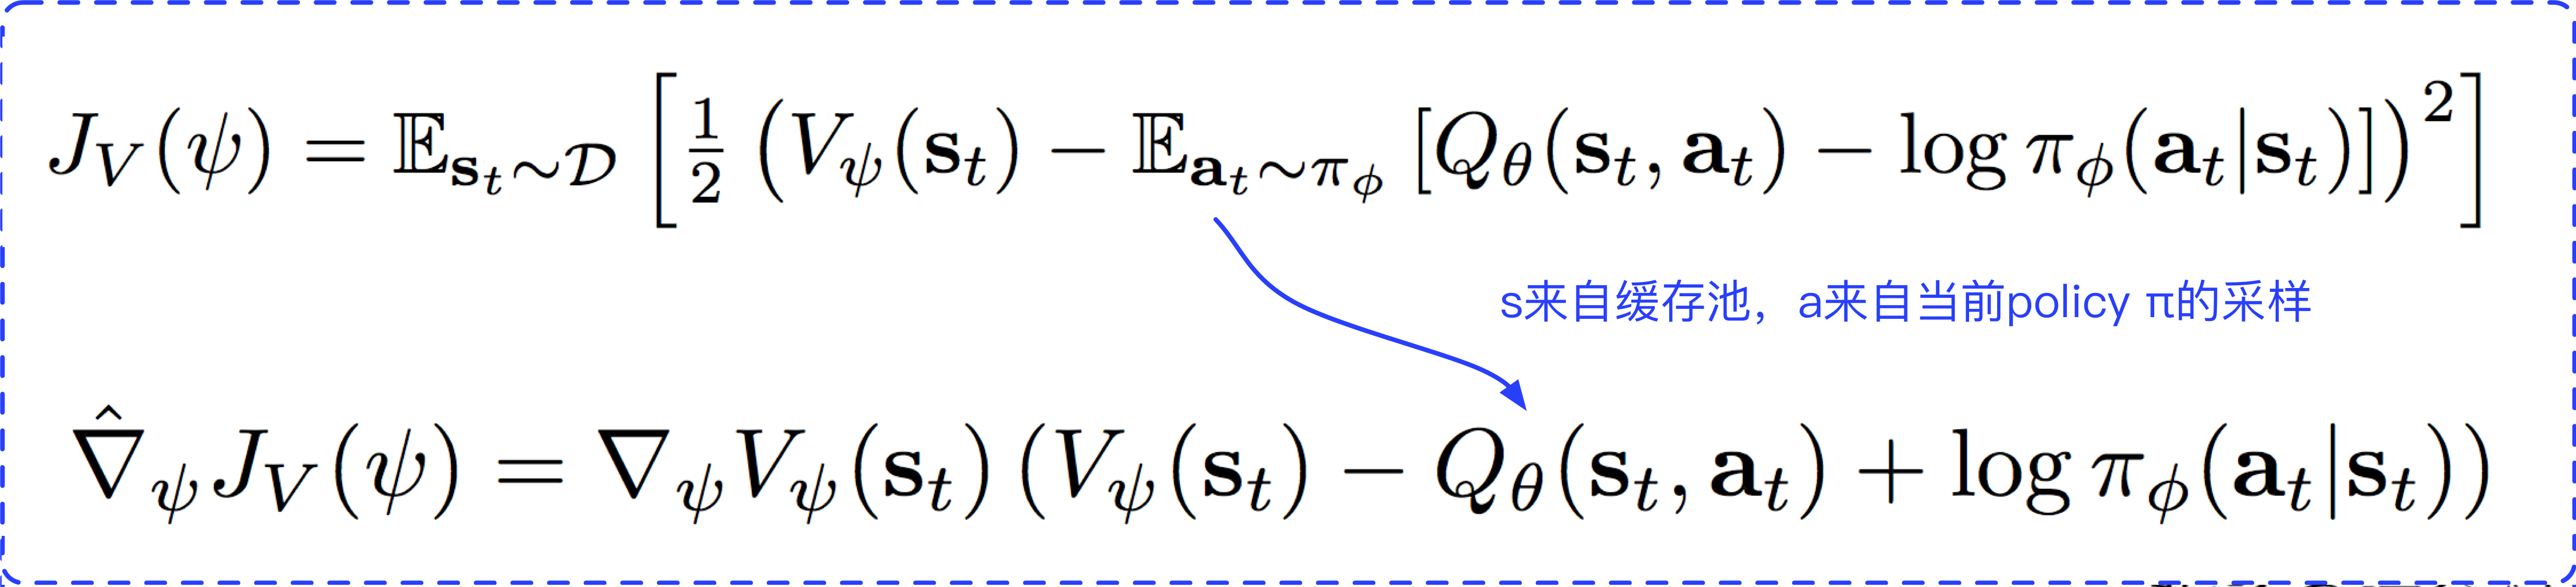
\includegraphics[scale=0.13]{pix/soft_state_value.png}
\caption{Soft state value}
%\label{fig:label}
\end{figure}


\subsection{Soft Q-Value 目标函数}

通过$V$近似$Q$,这里的$V$来自TargetNetwork $V$。
$r(s,a)$是环境的即时奖赏;$s_{t+1}$来自环境,由于环境是model-free,
可以理解成$s_{t+1}$是确定的。

\begin{figure}[!htb]
\centering
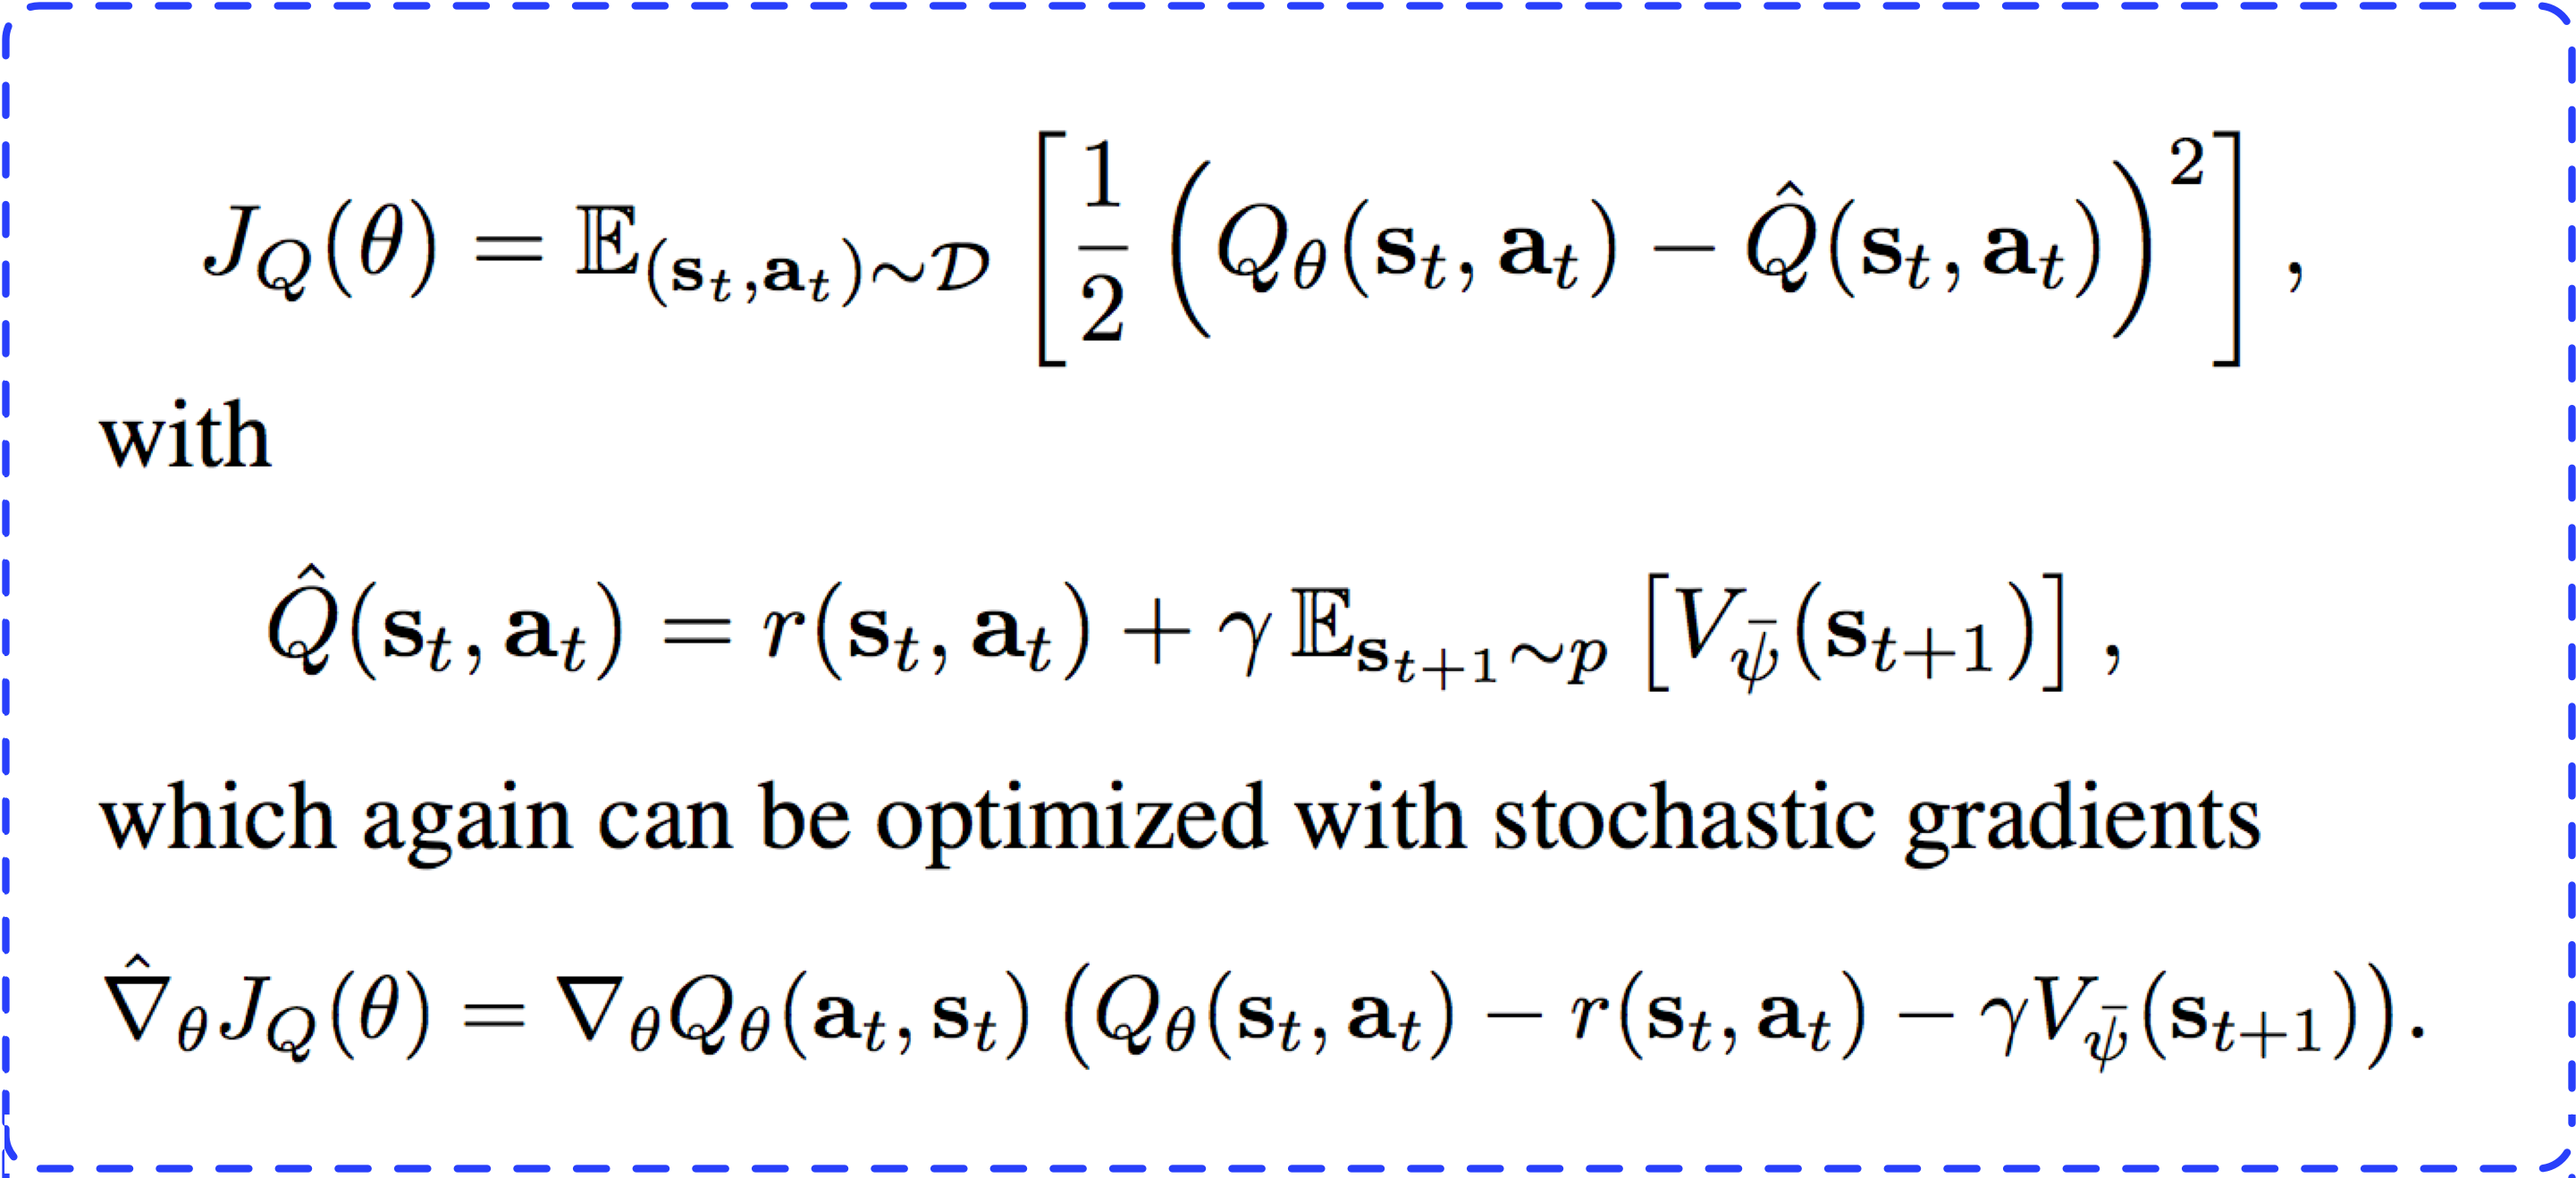
\includegraphics[scale=0.2]{pix/soft_q_value.png}
\caption{Soft Q value}
%\label{fig:label}
\end{figure}


\subsection{Policy 目标函数}

通过$Q$近似$\pi$。

\begin{itemize}
%\setlength{\itemsep}{0pt}
%\setlength{\parsep}{0pt}
\setlength{\parskip}{0pt}
\item[1.]
基于$\pi$分布的采样增加扰动,for lower variance estimator。

\item[2.]
KL散度基于$Q$的分布近似忽略分母析分函数。

\item[3.]
采样之后,$a$是确定的,KL散度即熵的差容易求解,注意$Q$值来自神经网络,值可以scale,无需关注系数。
\end{itemize}

\begin{figure}[!htb]
\centering
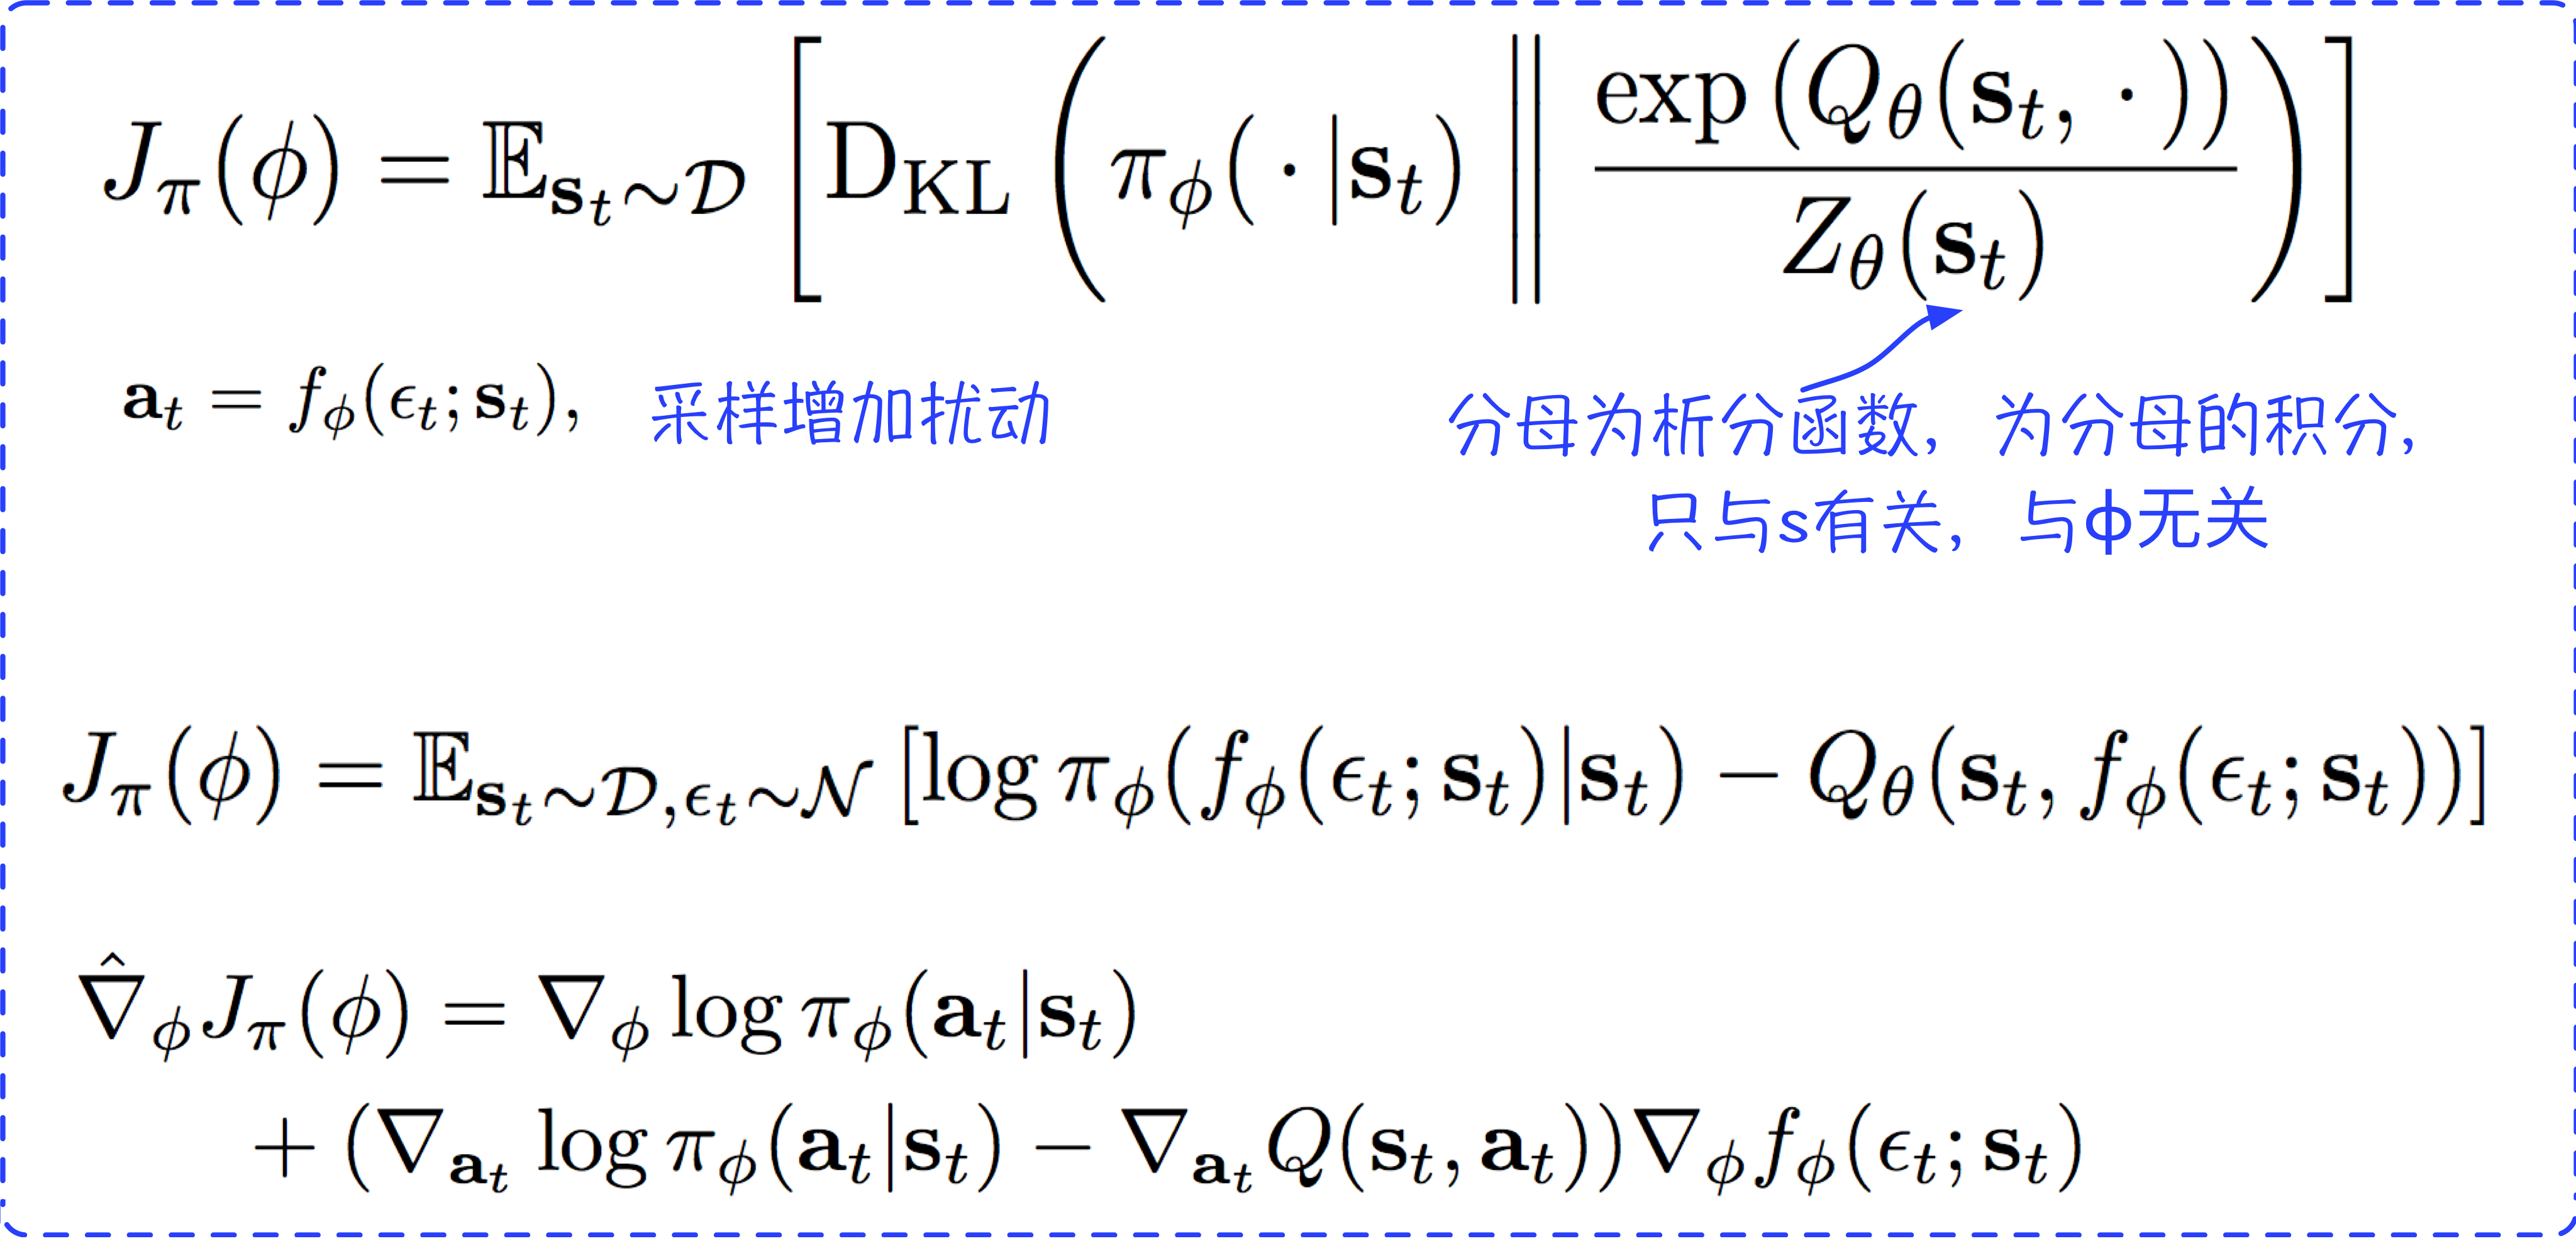
\includegraphics[scale=0.15]{pix/policy_objective.png}
\caption{Policy objective function}
%\label{fig:label}
\end{figure}


\subsection{学习过程}

整体采用Replay Buffer,三个目标函数分别进行梯度学习。

\begin{figure}[!htb]
\centering
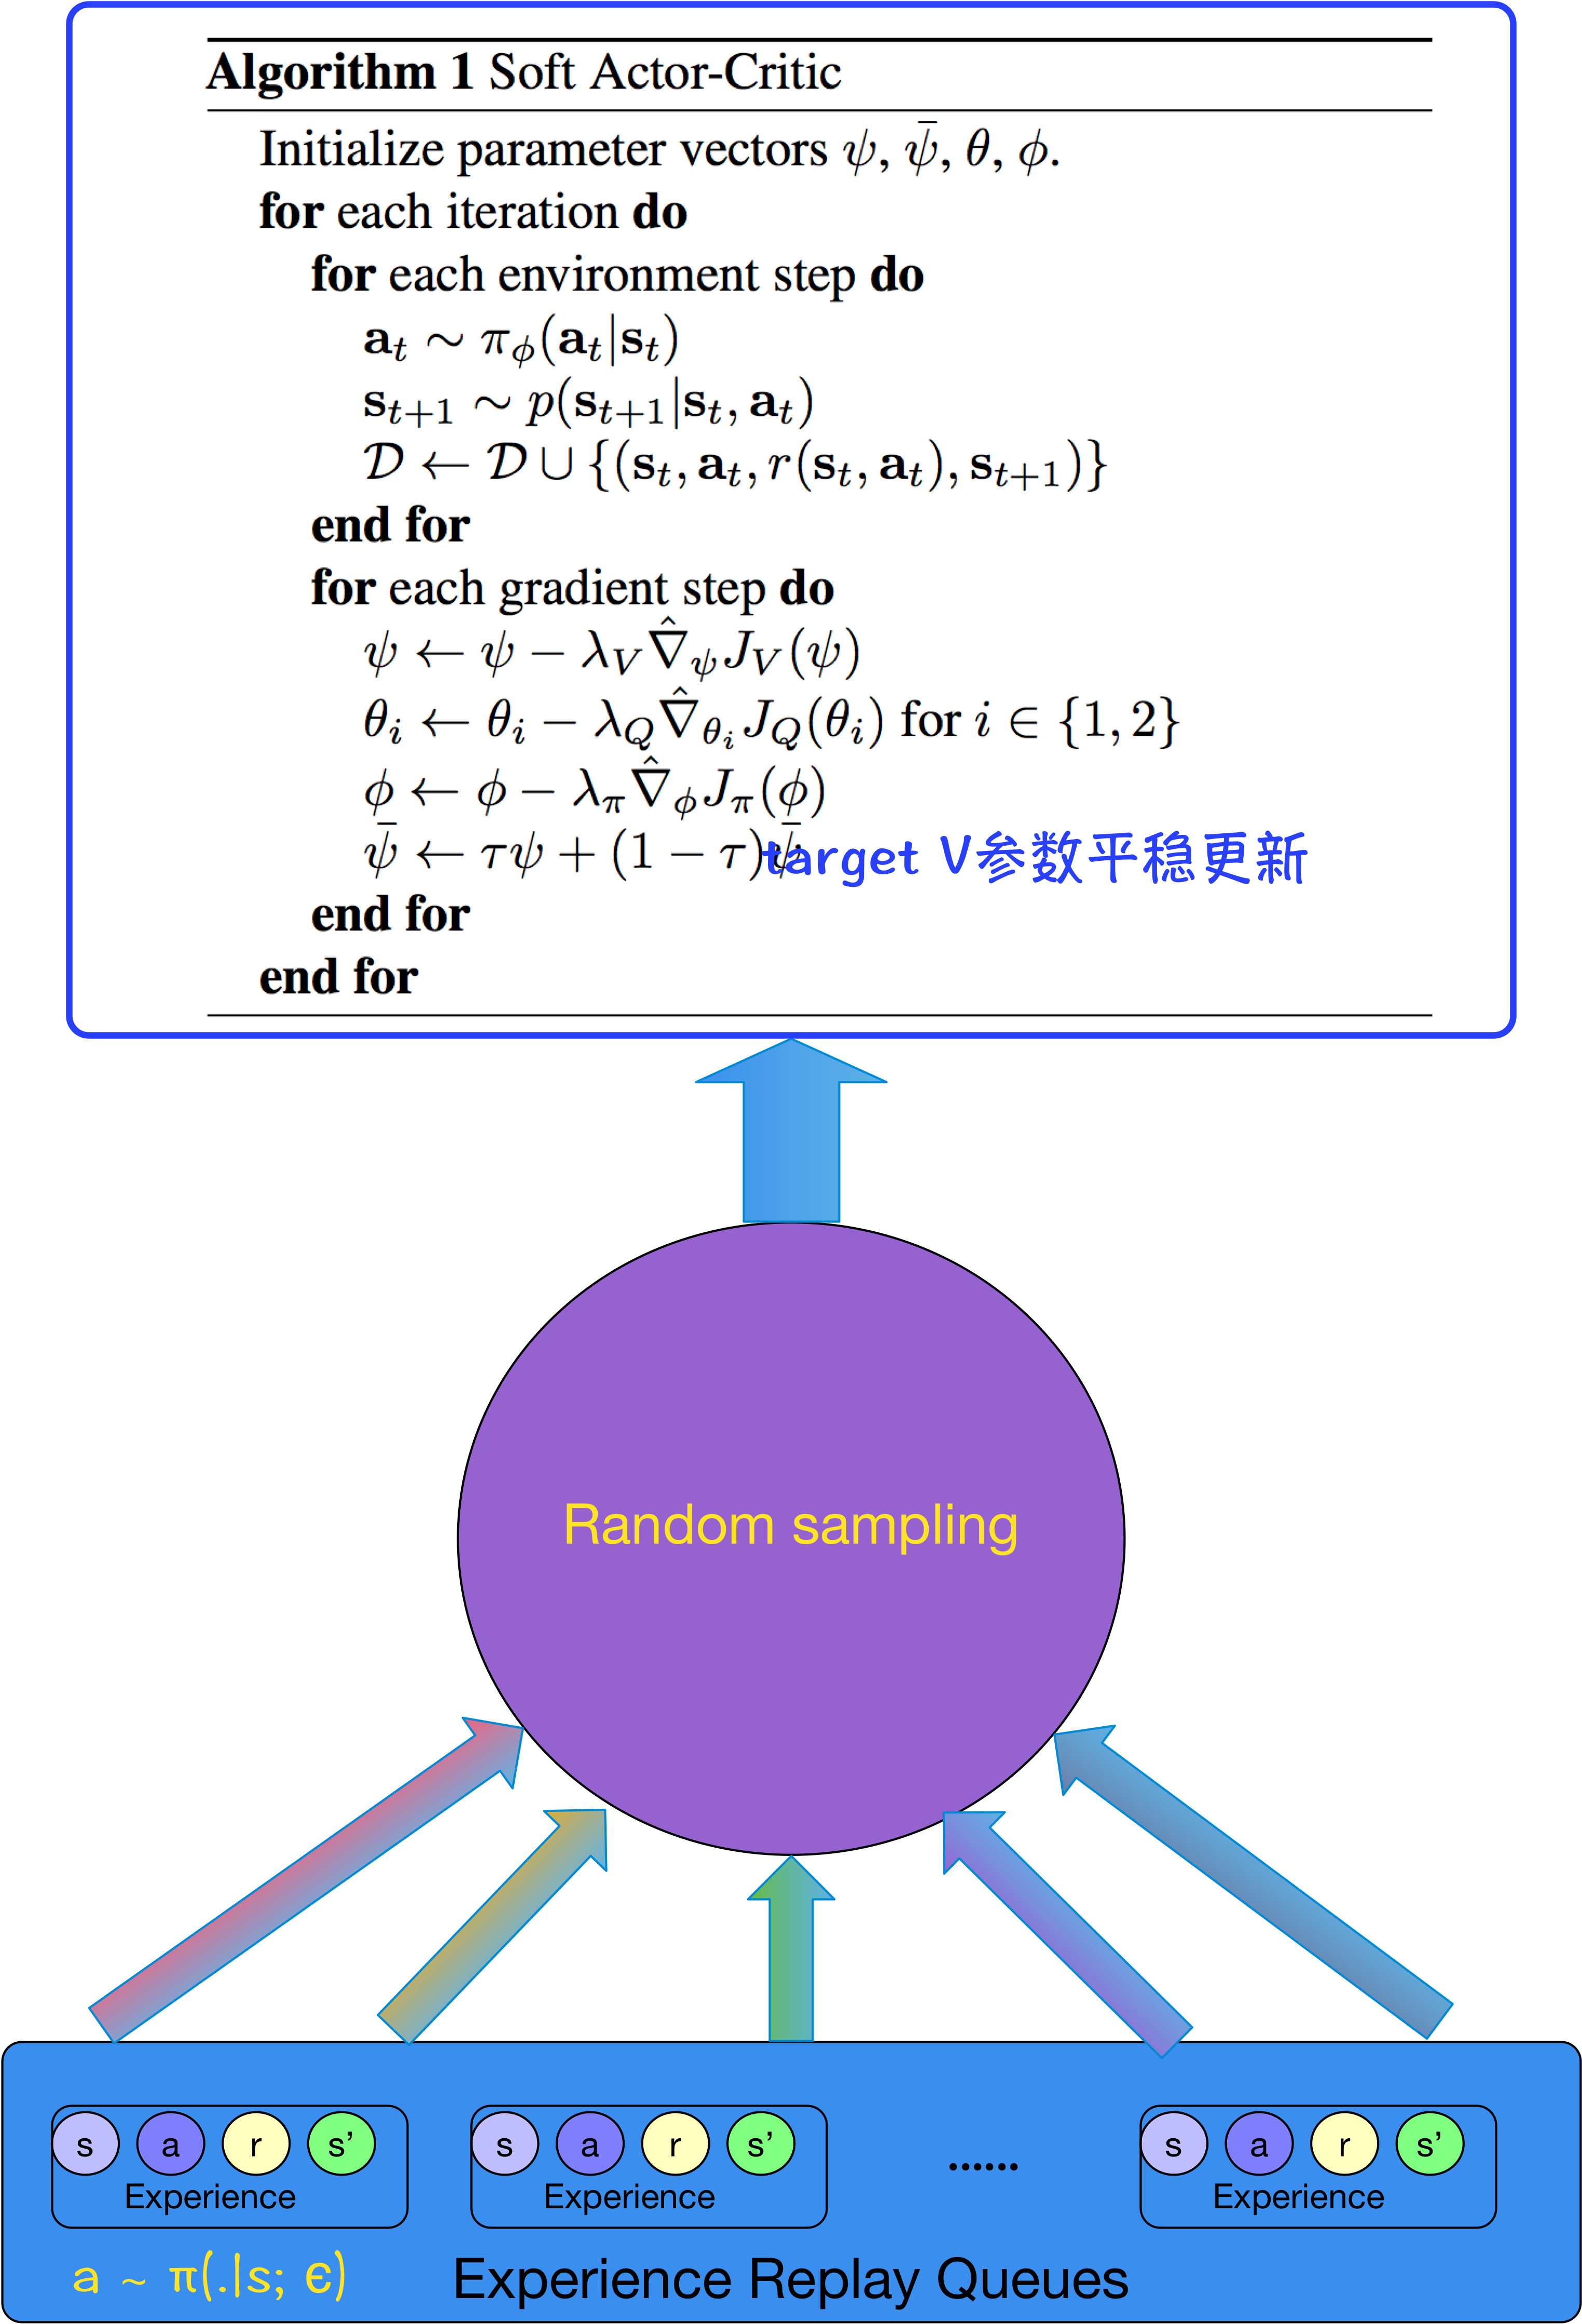
\includegraphics[scale=0.15]{pix/learning_process.png}
\caption{Learning process}
%\label{fig:label}
\end{figure}


\subsection{总结}

\begin{itemize}
%\setlength{\itemsep}{0pt}
%\setlength{\parsep}{0pt}
\setlength{\parskip}{0pt}
\item[1.]
SAC的关键是引入{\bf 最大熵},优化soft value。

\item[2.]
最大熵会使action{\bf 探索能力很强},模型效果更平稳,但注意需要场景也是接受较强的探索。

\item[3.]
从结构上讲,{\bf 模型冗余},在学习$\pi$和soft $Q$的情况下,又学习了soft $V$。

\item[4.]
由于面临的是连续动作空间,求期望的地方,采取了{\bf 采样近似},需要批次处理的数据集更加完整。

\item[5.]
优化技巧比较晦涩,感觉很难通用
\end{itemize}
